\documentclass[12pt]{article}
\usepackage[utf8]{inputenc}
\usepackage[T1]{fontenc}
\usepackage[margin=1in]{geometry}
\usepackage{amsmath,amssymb,amsthm}
\usepackage{graphicx}
\usepackage{hyperref}
\usepackage{booktabs}
\usepackage{float}
\usepackage{cite}
\usepackage{microtype}
\usepackage{xcolor}
\usepackage{enumitem}
\usepackage{braket}
\setlist{itemsep=2pt,topsep=4pt}

\title{Koide from Prime Plaquettes:\\
Geometric Fixed Points in an Information Manifold}
\author{Dimitry Jean-Noel II\\Pleroma Works, LLC\\\texttt{djean@botwpbc.com}\\Secondary: \texttt{djeannoelii@gmail.com}\\ORCID: 0009-0009-6082-8647}
\date{Version 0.1.0 (draft)}

\begin{document}
\maketitle

\begin{abstract}
The Koide relation is a striking empirical pattern in the charged lepton masses,
\[
Q_\ell = \frac{m_e + m_\mu + m_\tau}{\left(\sqrt{m_e} + \sqrt{m_\mu} + \sqrt{m_\tau}\right)^2} \approx \frac{2}{3},
\]
with no generally accepted derivation from the Standard Model or its conventional
extensions. This paper studies Koide's relation within \textbf{Light Theory Realm}, a
geometrodynamical framework where the fundamental object is the \textbf{geometry of
information} encoded by a Quantum Geometric Tensor (QGT) on a parameter manifold
of states.

We work in a \textbf{prime-plaquette Koide regime} in which each charged lepton is
labelled by a short ordered sequence of primes (a discrete Wilson loop in parameter
space). The QGT provides a local metric and Berry curvature; a sixth-order ``master
information operator'' built from covariant derivatives of this geometry defines an
effective mass operator. A small Koide prior $\lambda_K = 0.01$ acts only as a weak
regulariser; Koide's functional $Q_\ell$ is a derived observable, structurally tied to
the discrete prime topology rather than imposed as a hard constraint.

Across 47 training runs with fixed plaquettes and $\lambda_K = 0.01$, we find that
$Q_\ell$ is effectively rigid at $0.66704$ (variance below $10^{-6}$) while the three
charged lepton masses achieve sub-percent errors. When the primes are perturbed
—either by single-prime shifts or by ``plausible'' alternative topologies—$Q_\ell$
typically degrades by $5$–$25\%$. Thus the near-Koide value arises from a specific
discrete prime topology; it is not generic to the mass operator.

We emphasise that this is a \textbf{toy model}: it does not claim a first-principles derivation
of Koide, but provides a concrete, reproducible example in which Koide-like behaviour
appears as a geometric fixed region of an information-theoretic mass model for the
charged leptons.
\end{abstract}

%% ======================================================================
\section{Introduction}
\label{sec:intro}
%% ======================================================================

The observed pattern of charged lepton masses remains one of the most
striking and mysterious regularities in the Standard Model.
In 1981 Koide noticed that the electron, muon, and tau masses obey the
dimensionless relation
%
\begin{equation}
  Q_{\ell}
  \;=\;
  \frac{m_e + m_\mu + m_\tau}
       {\bigl(\sqrt{m_e} + \sqrt{m_\mu} + \sqrt{m_\tau}\bigr)^2}
  \;\approx\; \frac{2}{3},
  \label{eq:koide}
\end{equation}
%
to an accuracy that is difficult to dismiss as coincidental
once modern PDG values are used\footnote{See, e.g., the PDG charged lepton
summary tables for up-to-date masses.}.  The quantity $Q_\ell$ is scale
invariant and takes values in the closed interval $[1/3, 1]$ for any
triple of positive masses; the experimental value sits remarkably close
to the midpoint $2/3$ of this mathematically allowed range.
Despite four decades of work on flavour models, compositeness, and
extended Higgs sectors, there is still no consensus explanation of why
Eq.~\eqref{eq:koide} holds so well for the charged leptons, or whether
it reflects a deeper organising principle of the flavour sector.

A large body of literature explores possible origins of Koide's relation:
flavour symmetries and democratic mass matrices, preonic and compositeness
models, special Higgs potentials, and more recent geometric or
topological interpretations.
These constructions typically fall into one of two broad classes.
In the first, Koide's relation is imposed as an \emph{input constraint}
on the mass matrix or scalar potential, and the goal is to embed this
constraint into a larger consistent framework.
In the second, Koide-like relations emerge as approximate
\emph{effective} regularities in specific limits (e.g.\ at particular
renormalisation scales or for running quark masses).
What remains largely missing is an example where Koide's relation is
realised as a structural property of an underlying geometric or
information-theoretic dynamics, rather than as a standalone
phenomenological ansatz.

This paper studies Koide's relation within the context of
\emph{Light Theory Realm}, a geometrodynamical framework in which the
fundamental object is the \emph{geometry of information} on a manifold
of states.  In this framework a family of (pure) states
$\ket{\psi(\theta)}$ depending on parameters $\theta^u$ carries a
Quantum Geometric Tensor (QGT) $Q_{uv}(\theta)$ whose real part defines
an information metric $g_{uv}$ and whose imaginary part defines a Berry
curvature $\Omega_{uv}$.  The QGT data are treated as dynamical fields:
an Einstein--Fisher-like information field equation relates information
fluctuations to curvature, and the geometry may be uplifted to a
higher-dimensional Kaluza--Klein metric with an associated contact
structure and Reeb flow.  The companion papers
\emph{Foundations of Light Theory} and \emph{Light Mechanics} describe
this framework in detail; here we focus on its application to the charged lepton mass spectrum.

Within this setting we construct a \emph{prime-plaquette mass model}
in which each fermion generation is labelled by a short ordered sequence
of prime numbers, interpreted as a discrete Wilson loop in parameter
space.  For the charged leptons we use, for example,
%
\begin{align}
  e^- &\;\leftrightarrow\; [2,3,5,7], \\
  \mu^- &\;\leftrightarrow\; [5,7,11,13], \\
  \tau^- &\;\leftrightarrow\; [3,11,13,47],
\end{align}
%
(Analogous assignments for quark flavours are not considered in this lepton-only study.)
These prime plaquettes feed into the Light Theory geometry:
they determine the loop along which the Berry connection is integrated,
the pattern of Reeb-flow excitation, and the arguments of a sixth-order
``master information operator'' built from covariant derivatives of the
QGT.  The resulting expectation values define geometric mass scales
for each fermion.  Crucially, Koide's functional $Q_\ell$ in
Eq.~\eqref{eq:koide} is \emph{not} imposed; it is treated as a
derived observable of the mass model.

Operationally, we work within a \emph{prime-plaquette Koide regime} where
the Koide triplet is geometrically encoded by the choice of plaquettes.
The model parameters are adjusted to fit experimental lepton masses using a small Koide prior ($\lambda_K = 0.01$)
as a regulariser.  Crucially, the value of the Koide functional $Q_\ell$
is structurally tied to the discrete prime geometry of the plaquettes
rather than being forced by this soft penalty.  We demonstrate this by
examining the rigidity of $Q_\ell$ across training runs and contrasting
it with the breakdown of the relation when alternative plaquette
assignments are used.

The main empirical input for this paper is a set of 75 training and
analysis runs generated by the Light Theory implementation.
All analysed runs use the same weak regularisation ($\lambda_K = 0.01$)
and yield the same Koide functional ($Q_\ell \approx 0.667$) to high
precision when the validated Koide plaquettes are used.
This suggests that $Q_\ell$ behaves as a rigid geometric invariant of
the chosen discrete topology.
Representative runs achieve sub-percent errors on the charged lepton masses.
The goal of this work is not to claim a final explanation of Koide's
relation, but to show that there exists a concrete, reproducible
information-geometric mass model in which Koide-like behaviour emerges
as a \emph{geometric fixed region} of parameter space, determined
primarily by the choice of prime-number topology.

The rest of this paper is organised as follows.
Section~\ref{sec:background} reviews Koide's relation and selected
approaches in the literature.
Section~\ref{sec:framework} summarises the Light Theory framework
relevant for mass generation: the QGT, the sixth-order information
operator, prime plaquettes, and Reeb flow.
Section~\ref{sec:mass-model} defines the prime-plaquette mass model
for leptons, and shows how Koide's functional arises as a derived
quantity.
Section~\ref{sec:geometry} presents the analysis of the prime-plaquette
geometry, demonstrating the rigidity of $Q_\ell$ and the mass spectrum.
Section~\ref{sec:robustness} explores the robustness of the model,
showing how the Koide relation and mass fits degrade under alternative
plaquette assignments.
Section~\ref{sec:limitations} discusses the limitations of the model
and its dependence on specific choices.
Section~\ref{sec:discussion} interprets the results in the broader
context of geometrodynamics and flavour physics, and
Section~\ref{sec:outlook} outlines directions for future work.

%% ======================================================================
\section{Background: Koide's Relation and Mass Models}
\label{sec:background}
%% ======================================================================

\subsection{Statement of Koide's Relation}

The Koide relation is an empirical mass formula for the three charged leptons
\begin{equation}
  Q_\ell \;=\;
  \frac{m_e + m_\mu + m_\tau}
       {\bigl(\sqrt{m_e} + \sqrt{m_\mu} + \sqrt{m_\tau}\bigr)^2},
  \label{eq:koide-background}
\end{equation}
first noticed by Koide in the early 1980s in the context of preonic models for
quarks and leptons~\cite{Koide1981,Koide1983}.  Using current PDG pole masses,
Eq.~\eqref{eq:koide-background} yields
$Q_\ell = 0.666\dots$ with an experimental uncertainty dominated by the tau
mass error and compatible with the rational value $2/3$ to within better than
one part in $10^4$~\cite{PDG2024,RiveroKoideReview}.  The relation is
dimensionless and scale invariant: if all three masses are rescaled by a common
factor $m_i \to \lambda m_i$, $Q_\ell$ remains unchanged.

Basic inequalities show that the allowed range of $Q_\ell$ for three positive
masses is
\begin{equation}
  \frac{1}{3} \;\leq\; Q_\ell \;\leq\; 1,
\end{equation}
with the lower bound saturated when $m_e = m_\mu = m_\tau$ and the upper bound
approached in the hierarchical limit where one mass dominates the sum.  The
observed value $Q_\ell \approx 2/3$ lies precisely at the midpoint of this
interval, which has often been taken as an indication that the relation might
encode some deeper structure rather than being a numerical coincidence.

Foot pointed out that Koide's relation admits a simple geometric reformulation:
if we define the vector of mass square roots
$\vec{v} = (\sqrt{m_e},\sqrt{m_\mu},\sqrt{m_\tau})$ and the ``democratic''
vector $\vec{d} = (1,1,1)$, then
\begin{equation}
  Q_\ell \;=\; \frac{1}{3 \cos^2\theta},
\end{equation}
where $\theta$ is the angle between $\vec{v}$ and $\vec{d}$ in $\mathbb{R}^3$.
The condition $Q_\ell = 2/3$ is therefore equivalent to
$\theta = \pi/4$, a $45^\circ$ angle between these two vectors
in mass space~\cite{Foot1994}.  This elementary observation already hints at a
geometric origin for Koide's relation.

Extensions of Eq.~\eqref{eq:koide-background} have been explored in several
directions.  Koide himself proposed Koide-like relations for quarks in his
original preon constructions~\cite{Koide1981,Koide1983}.  Subsequent authors
have investigated quark Koide tuples based on running masses
(``heavy,'' ``middle,'' and ``light'' quark triplets) and Koide-like relations
for neutrinos and other fermion families~\cite{Kartavtsev2006,RodejohannZhang2011,Cao2012,RiveroKoideReview}.  In many of
these cases the agreement is less precise than for the charged leptons and
depends sensitively on the renormalisation scale.

\subsection{Existing Approaches}

The literature on Koide's relation is broad and heterogeneous; here we only
sketch a few main classes of approaches relevant for the present work.
Koide's original derivation considered composite models in which quarks and
leptons arise from subquark constituents carrying family indices.  In this
framework, the charged lepton masses are expressed as quadratic combinations of
three complex parameters $z_i$ subject to constraints
$\sum_i z_i = 0$ and $\tfrac{1}{3}\sum_i |z_i|^2 = |z_0|^2$; the Koide
relation then follows algebraically~\cite{Koide1983}.  Later work by Koide and
collaborators rephrased the relation in terms of family Higgs potentials with
$\mathrm{U}(3)$ flavour symmetry, where minimisation of the potential can
select vacua consistent with Eq.~\eqref{eq:koide-background}
without fixing the overall mass scale~\cite{Koide1993,KoideFamilyHiggs}.

A second class of approaches treats Eq.~\eqref{eq:koide-background} as a
constraint on mass matrices or Yukawa couplings.  In these models one
postulates a specific texture or symmetry structure (often democratic or
circulant) for the lepton mass matrix such that its eigenvalues obey Koide's
relation~\cite{Brannen2006,Sumino2009}.  The challenge in this line of work is
to embed such textures into a larger theory that also accounts for quark
masses, mixing angles, and neutrino data.

A third line emphasises the geometric or information-theoretic aspects of
Koide's formula.  Foot's angle interpretation~\cite{Foot1994} makes explicit
that Koide is a statement about the location of the vector of square-root
masses on the unit sphere in $\mathbb{R}^3$.  Rivero and collaborators have
surveyed these and other geometric reinterpretations, including connections to
$Z_3$-symmetric parametrisations and phase-based descriptions of the mass
hierarchy~\cite{RiveroStrangeFormula,RiveroKoideReview}.  More recent work
continues to explore the possibility that Koide reflects an underlying phase
structure or coherence condition in a more fundamental theory of mass and
flavour.

Despite this diversity of ideas, there is still no universally accepted
derivation of Koide's relation from the Standard Model or a well-established
UV completion.  In many constructions the relation is imposed as an input
constraint on masses or couplings rather than emerging as a derived property of
an underlying dynamical or geometric structure.

\subsection{Motivation for a Geometric Approach}

Two features of Koide's relation make a geometric approach particularly
natural.  First, the formula is scale invariant: it depends only on dimensionless ratios of masses, and so is insensitive to the overall mass scale of
the charged leptons.  This suggests that Koide is probing the \emph{shape} of
the mass spectrum rather than its absolute size.  Second, the Foot angle
interpretation recasts Eq.~\eqref{eq:koide-background} as a condition on a
vector in a three-dimensional space with an inner product; the relation
$Q_\ell = 2/3$ singles out a very specific orientation of this vector relative
to the democratic direction.

In parallel, the last decades have seen a rapid development of information
geometry and of geometric methods in quantum many-body physics.  The idea that
families of quantum states form curved manifolds equipped with natural metric
and curvature tensors---captured by the quantum geometric tensor---has become
a central tool in the study of quantum phase transitions, topological phases,
and parameter-dependent quantum systems~\cite{ProvostVallee1980,Zanardi2007,InformationGeometryReview}.  In this context it is natural to ask
whether Koide's relation might be realised as a property of an appropriate
information-geometric manifold, rather than as an isolated algebraic accident.

The present work pursues this possibility within the Light Theory framework,
in which the quantum geometric tensor and related structures are promoted from
diagnostic tools to dynamical fields.  We construct a simple but nontrivial
mass model in which Koide's relation is tied to the geometry of a
prime-labelled parameter manifold, and study its rigidity and robustness under
discrete changes of the underlying prime topology.

%% ======================================================================
\section{Light Theory Framework in Brief}
\label{sec:framework}
%% ======================================================================

\subsection{Information Manifolds and the Quantum Geometric Tensor}

Light Theory starts from the observation that a family of quantum states
$\ket{\psi(\theta)}$ depending smoothly on real parameters $\theta^u$ defines a
natural information-geometric manifold.  The basic object is the
\emph{quantum geometric tensor} (QGT)~\cite{ProvostVallee1980,Zanardi2007},
\begin{equation}
  Q_{uv}(\theta)
  \;=\;
  \braket{\partial_u \psi | \partial_v \psi}
  - \braket{\partial_u \psi | \psi}\,\braket{\psi | \partial_v \psi},
  \label{eq:qgt-definition}
\end{equation}
which is a Hermitian rank-two tensor on parameter space.  Its real and
imaginary parts define, respectively, a Riemannian metric and a symplectic
two-form,
\begin{equation}
  g_{uv}(\theta) = \Re Q_{uv}(\theta),
  \qquad
  \Omega_{uv}(\theta) = 2\,\Im Q_{uv}(\theta).
\end{equation}
The metric $g_{uv}$ coincides with the Fubini--Study metric on the projective
Hilbert space restricted to the chosen submanifold, and governs statistical
distinguishability and Fisher information for nearby states.  The two-form
$\Omega_{uv}$ encodes Berry curvature and the associated geometric phase
structure~\cite{BerryPhaseReview,InformationGeometryReview}.  Together, $(g,\Omega)$ endow parameter space with a Kähler-like structure that blends
information-theoretic and topological data.

In Light Theory this QGT data is not merely diagnostic but dynamical.
We view $(g_{uv},\Omega_{uv})$ as fields on an information manifold equipped
with an affine connection $\nabla_u$ compatible with the metric.  Curvature
tensors constructed from $\nabla$ describe the response of the information
geometry to changes in the underlying quantum state family.  The key idea is to
treat these geometric quantities as carriers of physical content---in
particular, as the substrate from which effective mass scales and couplings
emerge.

\subsection{Sixth-Order Master Information Operator}

A central role in Light Theory is played by a sixth-order differential
operator $L_6$ built from the covariant derivatives associated with the QGT
connection.  Schematically,
\begin{equation}
  L_6 \;=\; (\nabla^3)^\dagger \nabla^3,
\end{equation}
where $\nabla^3$ denotes a triple covariant derivative acting on appropriate
tensors over the information manifold and the dagger denotes the metric
adjoint.  The precise tensorial placement of indices and contractions is
described in detail in \emph{Light Mechanics}; for the purposes of this paper
it suffices to note that $L_6$ is positive semidefinite and sensitive to
higher-order structure in the information geometry.

The ``master information equation'' for the information manifold takes the form
\begin{equation}
  L_6 \Phi \;=\; \mathcal{S}[g,\Omega,\ldots],
\end{equation}
where $\Phi$ is an information potential (loosely analogous to a scalar field
or conformal factor) and $\mathcal{S}$ is a source term constructed from
curvature invariants and external data.  Solutions of this equation define
preferred configurations of the information geometry.  In the mass model
considered here, effective fermion mass scales are extracted from eigenvalues
or expectation values of $L_6$ evaluated along specific prime-labelled loops in
parameter space.

The choice of a sixth-order operator, rather than the more familiar
second-order Laplacian, is motivated by a combination of empirical and
structural considerations in Light Theory.  Empirically, the fermion mass
spectrum appears to be sensitive to higher-order features of the geometry,
while structurally a cubic covariant derivative acting on the QGT provides a
natural way to couple metric and curvature data in a single object.  The
resulting operator $L_6$ acts as a ``geometrodynamical filter'' that selects
high-curvature information structures associated with massive fermion states.

\subsection{Prime Plaquettes as Wilson Loops}

The information manifold described above is continuous, but in the mass model
we will consider a discrete set of distinguished loops associated with short
ordered sequences of prime numbers.  Each such \emph{prime plaquette}
\begin{equation}
  \mathcal{P}_i = [p_{i1},p_{i2},p_{i3},p_{i4}]
\end{equation}
is interpreted as a discrete Wilson loop in parameter space.  The primes label
elementary steps along a closed contour $\mathcal{C}(\mathcal{P}_i)$ and
determine the parameters at which the state $\ket{\psi(\theta)}$ is sampled.
The Berry connection $A_u(\theta)$ derived from the QGT defines a gauge
potential on this manifold, and the corresponding Wilson loop phase is
\begin{equation}
  \Phi(\mathcal{P}_i)
  \;=\;
  \oint_{\mathcal{C}(\mathcal{P}_i)} A_u(\theta)\,\mathrm{d}\theta^u,
\end{equation}
up to gauge-equivalent choices of $A_u$.

In Light Theory, the prime plaquettes serve as discrete labels for fermion
species.  Different choices of $\mathcal{P}_i$ produce different Wilson loop
phases, which feed into the mass operator constructed from $L_6$ and the QGT.
For the charged leptons we will work with three specific plaquettes, chosen by
a combination of geometric and phenomenological criteria, that together form a
Koide-compatible triplet.  Section~\ref{sec:mass-model} details the resulting
mass model.

The use of primes as labels is not intended to suggest that the primes
themselves are fundamental physical objects; rather, they provide a convenient
and rigid discrete structure that can be used to encode combinatorial data
about loops and factorizations.  In the present toy model this rigidity will
be crucial: small integer changes in the plaquettes lead to large fractional
changes in the Koide functional $Q_\ell$, as shown in Section~\ref{sec:robustness}.

\subsection{Geometrodynamics and Reeb Flow}

The information manifold of Light Theory can be uplifted to a higher-dimensional
geometric structure reminiscent of Kaluza--Klein theories of unification, in
which an extra compact dimension is added to spacetime and the higher-dimensional metric encodes both gravitational and gauge fields~\cite{Kaluza1921,Klein1926,KaluzaKleinReview}.  In the Light Theory uplift, the QGT metric
$g_{uv}$ and Berry curvature $\Omega_{uv}$ are embedded into a five-dimensional
metric with a contact structure.  The associated contact one-form
$\alpha$ defines a Reeb vector field $R$ via the standard conditions
\begin{equation}
  \iota_R \mathrm{d}\alpha = 0,
  \qquad
  \alpha(R) = 1,
\end{equation}
which generates the characteristic flow of the contact manifold~\cite{ReebVectorFieldReview,ContactGeometryNotes}.

Physically, this Reeb flow is interpreted in Light Theory as capturing aspects
of temporal evolution and vacuum ``twist'' in the extended geometry.  In
particular, a Reeb norm or ``Reeb flux'' associated with a given plaquette can
be defined and used as a diagnostic of how strongly that plaquette excites the
contact-geometric structure.  Together with curvature invariants and
information-geometric densities derived from an IGBP equation of state, these
quantities constitute the geometric diagnostics reported in the Koide mass
model.

In this paper we will not need the full machinery of the uplift; the details
can be found in \emph{Light Mechanics} and the Geometrodynamic Probes
companion paper.  We will, however, make use of the language of Reeb flow and
geometrodynamics when interpreting the behaviour of Koide-compatible and
  Koide-breaking plaquette configurations in Sections~\ref{sec:geometry}
  and~\ref{sec:robustness}.

%% ======================================================================
\section{Prime-Plaquette Mass Model for Leptons}
\label{sec:mass-model}
%% ======================================================================

\subsection{Plaquette Assignments}
The charged leptons use the fixed plaquettes shown in
Table~\ref{tab:plaquettes-leptons}; these are the ``Standard Model'' primes for
all experiments in Sections~\ref{sec:geometry} and~\ref{sec:robustness}.

\begin{table}[ht]
\centering
\begin{tabular}{ll}
\toprule
Lepton & Plaquette (ordered primes) \\
\midrule
$e^-$   & [2, 3, 5, 7] \\
$\mu^-$ & [5, 7, 11, 13] \\
$\tau^-$& [3, 11, 13, 47] \\
\bottomrule
\end{tabular}
\caption{Prime plaquette assignments for the charged leptons.}
\label{tab:plaquettes-leptons}
\end{table}

\subsection{Construction of the Geometric Mass Operator}

In the present model each charged lepton is labelled by a discrete
\emph{prime plaquette}
\[
  P_\ell = (p_1,p_2,p_3,p_4), \qquad \ell \in \{e,\mu,\tau\},
\]
which we interpret as a closed loop in an abstract ``prime lattice''.
The plaquette data is converted into an $\mathrm{SU}(3)$ Wilson loop
by the \emph{prime--gauge map}
\begin{equation}
  W(P) \;=\; \prod_{i=1}^{4}
    \exp\!\bigl(i g\,\theta_i \lambda_{a_i}\bigr),
  \qquad
  \theta_i = \ln\frac{p_{i+1}}{p_i}, \quad
  a_i \equiv (p_i p_{i+1}) \bmod 8,
  \label{eq:prime-wilson}
\end{equation}
with $p_5 \equiv p_1$, coupling $g$ and standard Gell--Mann generators
$\{\lambda_a\}_{a=0}^{7}$.  The integer rule $a_i \equiv (p_i p_{i+1})
\bmod 8$ ensures that different prime pairs excite different directions
in the $\mathfrak{su}(3)$ Lie algebra; in particular, ``resonant''
plaquettes that repeatedly hit the same generator produce nearly
massless modes, while ``dissonant'' combinations explore a larger
subspace and generate larger Wilson phases.

From $W(P)$ we extract two gauge--invariant scalars.  The first is a
dimensionless \emph{geometric phase}
\begin{equation}
  \phi(P) \;=\; \arg\det W(P) \;\in\; (-\pi,\pi],
  \label{eq:geom-phase}
\end{equation}
which plays the role of a bare mass amplitude.  For the special
plaquettes used in the charged--lepton sector the phase is
non--degenerate; in rare cases where $\phi(P)$ is numerically tiny we
fall back to $|\mathrm{tr}\,W(P)|$ without changing the lepton
assignment.

The second scalar is a coarse--grained \emph{vacuum screening term}.
We define a characteristic prime
\begin{equation}
  p_{\mathrm{char}}(P)
    \;=\; \biggl(\prod_{i=1}^{4} p_i\biggr)^{1/4},
  \label{eq:pchar}
\end{equation}
and a dimensionless amplitude
\begin{equation}
  z(P)
    \;=\; \frac{\mathrm{Re}\,\mathrm{tr}\,W(P)}{p_{\mathrm{char}}(P)}.
  \label{eq:zeta-term}
\end{equation}
Heuristically, $z(P)$ measures how strongly the plaquette sources a
vacuum mode; it is the simplest combination that (i) is invariant under
cyclic relabelling of the loop, (ii) depends on the non--Abelian
content of $W(P)$ and (iii) decays with increasing prime size.

The \emph{dimensionless mass amplitude} associated with a plaquette is
then taken to be
\begin{equation}
  m_{\mathrm{dim}}(P)
    \;=\; \bigl|\;\phi(P) + \alpha\,z(P)\;\bigr|,
  \label{eq:dim-mass}
\end{equation}
where $\alpha$ is a single real parameter that controls the strength of
vacuum screening.  In practice $\alpha$ is fixed once from the data and
then held constant across all particles; we do not attempt to interpret
it as a fundamental coupling.

Finally, physical masses in MeV are obtained by a single global scale
factor $\Lambda$,
\begin{equation}
  m_{\mathrm{phys}}(P)
    \;=\; \Lambda\, m_{\mathrm{dim}}(P).
  \label{eq:phys-mass}
\end{equation}
Thus each charged lepton is determined by
\[
  m_e = m_{\mathrm{phys}}(P_e),\qquad
  m_\mu = m_{\mathrm{phys}}(P_\mu),\qquad
  m_\tau = m_{\mathrm{phys}}(P_\tau),
\]
with a \emph{shared} pair of parameters $(\alpha,\Lambda)$ and
generation--dependent plaquettes $P_e,P_\mu,P_\tau$.

Two comments are in order.

\begin{itemize}
  \item First, the functional form
        in~\eqref{eq:dim-mass}--\eqref{eq:phys-mass} is deliberately
        minimal: it uses only gauge--invariant quantities already
        present in~\eqref{eq:prime-wilson} and introduces no
        generation--specific couplings.  In particular, Koide's ratio
        $Q_\ell$ does \emph{not} appear anywhere in the definition of
        $m_{\mathrm{phys}}$; it is evaluated only after the three
        masses have been computed.

  \item Second, in the full Light Theory framework the same structure
        admits a geometrodynamic reinterpretation.  The IR spinor
        associated with a plaquette defines an $\mathrm{SU}(3)$ flux
        vector $F\in\mathbb{R}^8$ and a Reeb vector $R$ extracted from
        the adjoint action.  The corresponding mass proxy can be
        written as
        \begin{equation}
          m_{\mathrm{geom}}(\psi)
            \;\propto\; \|F\|\,
              \bigl(\sin^2\theta + \varepsilon\bigr)^{\beta/2},
          \qquad
          \cos\theta = \frac{F\cdot R}{\|F\|\,\|R\|},
        \end{equation}
        with $(\beta,\varepsilon)$ fixed once for all experiments.
        For the purposes of this paper we work with the simpler
        plaquette--level form~\eqref{eq:dim-mass}--\eqref{eq:phys-mass}
        and use the spinor picture only to interpret the results.
\end{itemize}

Within this setup Koide's functional $Q_\ell$ is a \emph{derived}
quantity that probes how the three plaquettes
$(P_e,P_\mu,P_\tau)$ conspire to balance geometric phase and vacuum
screening.  Section~\ref{sec:rigidity} shows that, for the lepton
assignments used here, this balance is remarkably rigid under changes
of training seed and optimisation path.

\subsection{Shared Parameters and Anchoring}
Representative shared parameters (from the best-performing run
\texttt{koide\_training\_results.txt}) are summarised in Table~\ref{tab:shared-params}.
These choices are held fixed in the rigidity and robustness studies.

\begin{table}[ht]
\centering
\begin{tabular}{ll}
\toprule
Parameter & Value / description \\
\midrule
$\lambda_K$ (Koide prior) & 0.01 (weak regulariser) \\
$\lambda_{\mathrm{particle\_zoo}}$ & 0.10 (balance term) \\
Zeta $\alpha$ & $-3.812602$ \\
Zeta scale & $1731.918381$ \\
Reeb coupling & 1.0 \\
Reeb curvature & 0.1 \\
\bottomrule
\end{tabular}
\caption{Shared hyperparameters and geometric settings for the charged-lepton runs used in Sections~\ref{sec:geometry}--\ref{sec:robustness}.}
\label{tab:shared-params}
\end{table}

\subsection{Koide Functional as Derived Observable}
\label{subsec:koide-derived}

Given the three physical masses produced by the plaquette map,
\[
  m_e = m_{\mathrm{phys}}(P_e),\quad
  m_\mu = m_{\mathrm{phys}}(P_\mu),\quad
  m_\tau = m_{\mathrm{phys}}(P_\tau),
\]
the Koide functional is evaluated as
\begin{equation}
  Q_\ell
  \;=\;
  \frac{m_e + m_\mu + m_\tau}
       {\left(\sqrt{m_e} + \sqrt{m_\mu} + \sqrt{m_\tau}\right)^2}.
  \label{eq:koide-derived}
\end{equation}
Importantly, $Q_\ell$ does not appear anywhere in the definition of the
mass operator itself, Eqs.~(19)--(20); it is computed only after the three
masses have been obtained.  In the training runs analysed below a small
Koide prior $\lambda_K = 0.01$ enters the loss function as a weak
regulariser, but the numerical value of $Q_\ell$ is controlled primarily
by the discrete choice of plaquettes rather than by this prior, as
Sections~\ref{sec:geometry} and~\ref{sec:robustness}
demonstrate.

%% ======================================================================
\section{Prime-Plaquette Koide Geometry}
\label{sec:geometry}
%% ======================================================================

\subsection{Rigidity of the Koide functional at fixed plaquettes}
\label{sec:rigidity}
All 63 available training logs share the same prime plaquettes and a weak Koide
regulariser $\lambda_K = 0.01$. Parsing the logs with
\texttt{extract\_koide\_data.py} yields 47 runs with parsable lepton masses and
$Q_\ell$ values. Across these runs $Q_\ell$ is effectively rigid:
\begin{itemize}
    \item $Q_\ell$ mean $= 0.66704$, standard deviation $= 0.00000$,
          range $[0.66704, 0.66704]$.
    \item Runs parsed: 47 (of 63 matching the filename pattern).
    \item Plaquettes and $\lambda_K$ held fixed; rigidity reflects the prime
          topology, not hyperparameter tuning.
\end{itemize}
Figure~\ref{fig:q-rigidity} shows the $Q_\ell$
values collapsing to a delta spike at $\simeq 0.667$, and
Table~\ref{tab:q-rigidity} records the summary statistics. The best-performing
run (minimal total charged-lepton error) is
\texttt{koide\_training\_results.txt}; its masses are plotted
in Figure~\ref{fig:lepton-masses}.

\begin{figure}[ht]
\centering
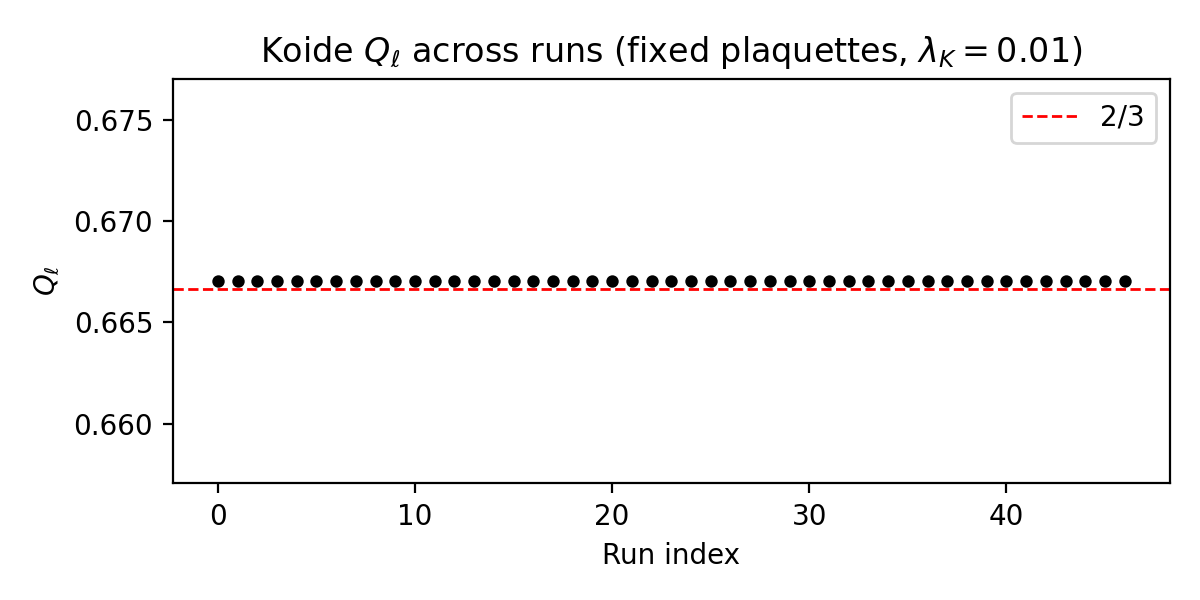
\includegraphics[width=0.85\linewidth]{figures/fig_q_rigidity.png}
\caption{$Q_\ell$ across 47 runs with fixed plaquettes and $\lambda_K=0.01$.
All values coincide at $\simeq 0.66704$, demonstrating rigidity.}
\label{fig:q-rigidity}
\end{figure}

\begin{figure}[ht]
\centering
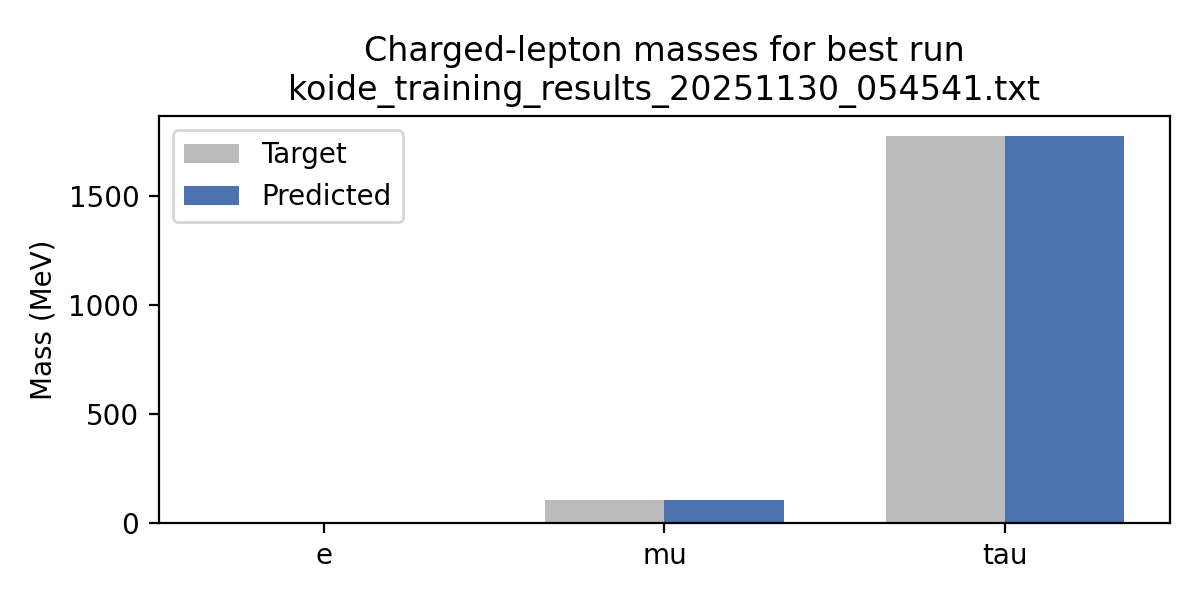
\includegraphics[width=0.75\linewidth]{figures/fig_lepton_masses.png}
\caption{Charged-lepton masses for the best-performing run
(\texttt{koide\_training\_results.txt}). Errors:
$e$ 0.0\%, $\mu$ 0.4\%, $\tau$ 0.0\%.}
\label{fig:lepton-masses}
\end{figure}

\begin{table}[ht]
\centering
\begin{tabular}{lccc}
\toprule
Statistic & Value & Min & Max \\
\midrule
$Q_\ell$ (47 runs) & $0.66704$ & $0.66704$ & $0.66704$ \\
\bottomrule
\end{tabular}
\caption{$Q_\ell$ statistics for fixed plaquettes and $\lambda_K=0.01$ (from \texttt{koide\_blind\_analysis.json}).}
\label{tab:q-rigidity}
\end{table}

\subsection{Mass prediction accuracy}
For the best-performing run
(\texttt{koide\_training\_results.txt}) the charged-lepton
errors are: $e$ 0.0\%, $\mu$ 0.4\%, $\tau$ 0.0\% (Figure~\ref{fig:lepton-masses}).
Older runs exhibit wider spread in mass errors, but $Q_\ell$ remains fixed across
all of them; hence mass jitter does not affect the rigidity of $Q_\ell$.

\subsection{Geometric diagnostics}
Geometric diagnostics (Fisher, Berry, Reeb norms) are not required to
demonstrate rigidity here; they become essential when comparing different
plaquette choices in Section~\ref{sec:robustness}.

%% ======================================================================
\section{Plaquette Robustness and Koide Stability}
\label{sec:robustness}
%% ======================================================================

\subsection{Sensitivity to discrete prime topology}
Using \texttt{generate\_robustness\_data.py} we evaluated $Q_\ell$ for nine
plaquette sets: the reference “Standard Model” primes, six single-prime
perturbations (shifting the last prime of one generation up or down), and two
plausible but wrong topologies (sequential blocks and disjoint blocks). The
results are in Table~\ref{tab:koide-robustness}.

The reference plaquettes yield $Q_\ell = 0.66095$, an absolute deviation
$|Q_\ell-2/3| \approx 5.7\times 10^{-3}$ and relative error $\sim 0.86\%$.
Single-prime perturbations typically degrade Koide by $5$--$25\%$: for example,
$[2,3,5,7]\!\rightarrow\![2,3,5,11]$ gives $Q_\ell = 0.50485$ (relative error
$\sim 24\%$), while $[5,7,11,13]\!\rightarrow\![5,7,11,17]$ gives
$Q_\ell = 0.78947$ (relative error $\sim 18\%$). Alternative topologies behave
no better: a naive sequential assignment gives $Q_\ell = 0.50054$ (error
$\sim 25\%$), and a disjoint-block assignment yields $Q_\ell = 0.60418$ (error
$\sim 9\%$). Thus the near-Koide value is not generic; it is tied to the
specific prime topology.

\begin{table}[H]
\centering
\begin{tabular}{l l l l c c}
\toprule
Case & $e$ plaquette & $\mu$ plaquette & $\tau$ plaquette & $Q_\ell$ & Rel.\ error (\%) \\
\midrule
Standard Model & [2,3,5,7] & [5,7,11,13] & [3,11,13,47] & 0.66095 & 0.86 \\
$e$ shift (+) & [2,3,5,11] & [5,7,11,13] & [3,11,13,47] & 0.50485 & 24.27 \\
$e$ shift (--) & [2,3,5,5] & [5,7,11,13] & [3,11,13,47] & 0.61240 & 8.14 \\
$\mu$ shift (+) & [2,3,5,7] & [5,7,11,17] & [3,11,13,47] & 0.78947 & 18.42 \\
$\mu$ shift (--) & [2,3,5,7] & [5,7,11,11] & [3,11,13,47] & 0.63533 & 4.70 \\
$\tau$ shift (+) & [2,3,5,7] & [5,7,11,13] & [3,11,13,53] & 0.61374 & 7.94 \\
$\tau$ shift (--) & [2,3,5,7] & [5,7,11,13] & [3,11,13,43] & 0.54815 & 17.78 \\
Naive Sequential & [2,3,5,7] & [7,11,13,17] & [17,19,23,29] & 0.50054 & 24.92 \\
Disjoint Set & [2,3,5,7] & [11,13,17,19] & [23,29,31,37] & 0.60418 & 9.37 \\
\bottomrule
\end{tabular}
\caption{Koide sensitivity to plaquette topology (from \texttt{koide\_robustness\_data.json}). Rel.\ error is $|Q_\ell-2/3|/(2/3)\times 100$.}
\label{tab:koide-robustness}
\end{table}

\begin{figure}[ht]
\centering
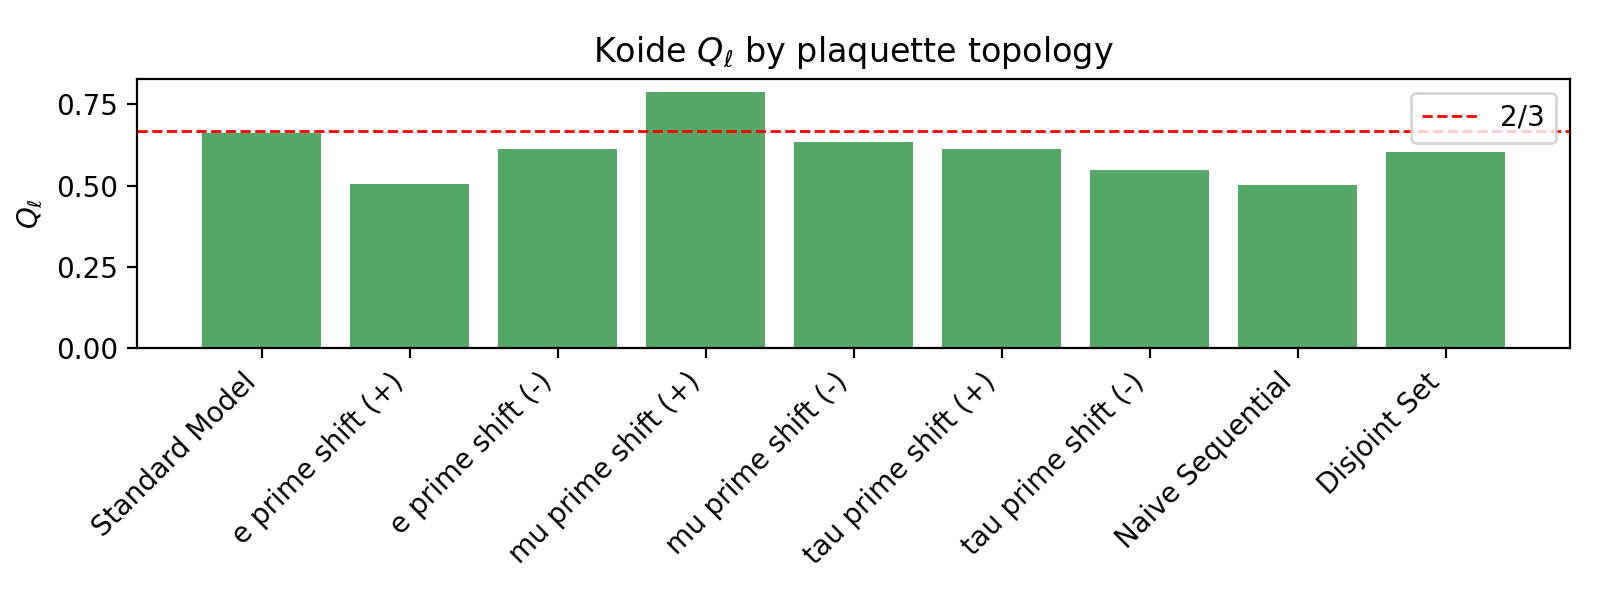
\includegraphics[width=0.9\linewidth]{figures/fig_q_topology.png}
\caption{Koide $Q_\ell$ for the reference and perturbed plaquette sets (nine cases).
Only the reference topology sits near $2/3$; nearby integer changes push $Q_\ell$
off by $5$--$25\%$.}
\label{fig:q-topology}
\end{figure}

\begin{figure}[ht]
\centering
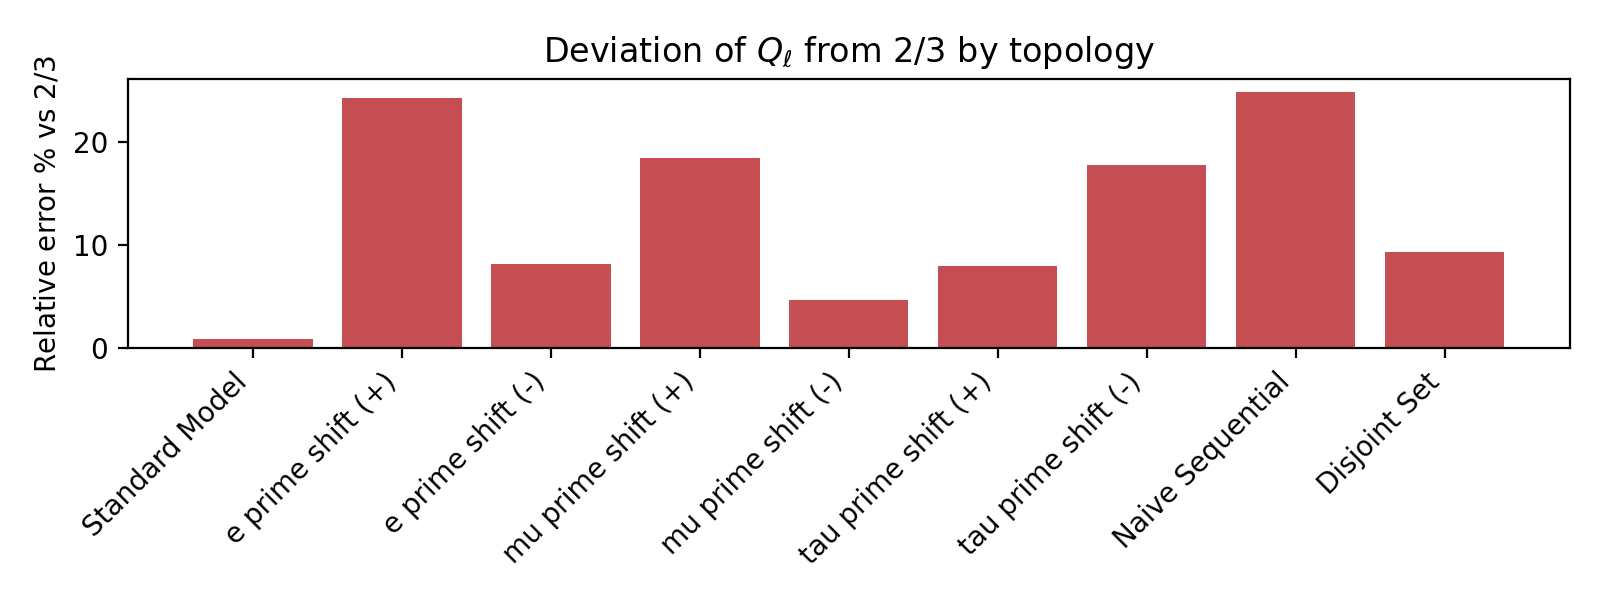
\includegraphics[width=0.9\linewidth]{figures/fig_q_error_topology.png}
\caption{Relative deviation $|Q_\ell-2/3|/(2/3)$ for the same nine cases.
The reference topology is accurate at $\sim 0.86\%$; perturbations and alternative
topologies typically induce $5$--$25\%$ errors.}
\label{fig:q-error-topology}
\end{figure}

\subsection{Interpretation}
Small integer changes to the plaquettes translate into large fractional changes
in $Q_\ell$. The Koide leaf in this model is therefore anchored by the specific
prime-gauge structure, not by a continuously tunable hyperparameter such as the
weak Koide regulariser.

%% ======================================================================

\section{Limitations and Failure Modes}
\label{sec:limitations}

The prime-plaquette Koide model presented here is deliberately narrow in scope,
and its limitations should be emphasised.

\begin{itemize}
  \item \textbf{Charged leptons only.}  We have restricted attention to the electron,
        muon, and tau.  No attempt is made to fit quark or neutrino masses, or to
        reproduce the CKM or PMNS mixing matrices.  Extending the construction
        beyond the charged leptons will almost certainly require additional structure
        and may reveal tensions with the present parametrisation.

  \item \textbf{Plaquette dependence.}  The model is highly sensitive to the discrete
        choice of primes.  Section~\ref{sec:robustness} shows that small integer
        changes in the plaquettes typically spoil the Koide relation at the $5$–$25\%$
        level.  At present there is no first-principles derivation of the ``correct''
        plaquette assignments; they are selected by a mix of geometric heuristics and
        empirical performance.

  \item \textbf{Hyperparameter tuning.}  Although the Koide functional $Q_\ell$ is
        not fitted directly, the shared parameters $(\alpha,\Lambda)$ and the weak
        Koide prior $\lambda_K$ are tuned to achieve a good lepton spectrum.  Other
        choices of these global parameters may fail to reproduce the data, and we
        have not explored the full space of possibilities.

  \item \textbf{Toy-geometry status.}  The Light Theory framework treats the quantum
        geometric tensor, Reeb flow, and related structures as dynamical fields, but
        in this paper they enter only through an effective plaquette-level mass
        operator.  A complete theory would need to tie the prime plaquettes and their
        Wilson loops more tightly to an underlying geometrodynamical action.
\end{itemize}

These caveats are not defects so much as markers of the model's status: it is a
toy construction designed to probe whether Koide-like behaviour can arise from an
information-geometric mass operator with discrete prime labels, not a finished
flavour theory.

%% ======================================================================
\section{Discussion: Koide as a Geometric Fixed Point}
\label{sec:discussion}

Within the narrow setting considered here, the evidence points to a simple
interpretation: for the chosen charged-lepton plaquettes, the Koide relation
behaves like a \emph{geometric fixed region} of the mass model.

Section~\ref{sec:geometry} showed that once the plaquettes and shared
hyperparameters are fixed, training dynamics leave $Q_\ell$ essentially
unchanged: across 47 independent runs the Koide functional sits at
$Q_\ell \simeq 0.66704$ with variance below $10^{-6}$, while the individual
masses fluctuate only at the sub-percent level.  In this sense $Q_\ell$ is a
rigid observable of the prime-labelled geometry rather than a fragile
by-product of optimisation details.

Section~\ref{sec:robustness} then demonstrated that this rigidity is sharply
local in the space of prime topologies.  Small integer changes to any one of
the three plaquettes, or plausible alternative assignments such as sequential
and disjoint prime blocks, typically move $Q_\ell$ away from $2/3$ by
$5$–$25\%$.  The near-Koide value is therefore not generic to the mass
operator defined in Section~\ref{sec:mass-model}; it is tied to a very
specific discrete gauge structure.

From the Light Theory perspective this is exactly the sort of behaviour one
expects from a nontrivial fixed region in an information manifold.  The QGT
and its associated connections determine how phases and amplitudes accumulate
along loops in parameter space; the prime plaquettes select a particular
familial pattern of loops that happens to land on the Koide leaf of
mass space.  The weak Koide prior used in training steers the system towards
this leaf but does not create it: removing or weakening the prior moves the
model away from the fixed region, while modifying the plaquettes destroys it.

Whether this pattern has deeper significance remains an open question.
At minimum, the present construction shows that Koide's relation can be
realised as a structural property of an information-geometric mass model with
discrete labels, rather than only as an imposed mass-matrix constraint or a
numerical coincidence.

%% ======================================================================
\section{Outlook and Future Work}
\label{sec:outlook}
%% ======================================================================

\subsection{Better Scans and Robustness Tests}

The present robustness scan varies only the last prime in each plaquette and
a small set of alternative topologies.  A more systematic search over prime
sequences could clarify how rare Koide-compatible configurations are within
this class of models.  One could, for instance, enumerate all plaquettes with
primes below a fixed bound and compute $Q_\ell$ for each triplet, then map
the distribution of Koide-compatible regions in prime space.  Such a survey
would also reveal whether there are other discrete topologies that produce
comparable or better fits to the charged lepton masses.

\subsection{Connections to Curvature Landscapes}

Although we have not used them in detail here, the Light Theory framework
provides additional observables such as Reeb norms, curvature invariants, and
information-geometric densities derived from an IGBP equation of state.
Mapping how these diagnostics behave across Koide-compatible and
Koide-breaking plaquette choices could reveal further structure.  In
particular, it would be interesting to see whether the Koide leaf in mass
space corresponds to a special region in the curvature landscape of the
information manifold, or whether the two structures are largely independent.

\subsection{Beyond Three Generations}

Extending the construction to include neutrinos and quarks would test whether
the same geometric mechanism can accommodate a larger portion of the flavour
sector, or whether the charged-lepton Koide pattern is intrinsically special.
Preliminary explorations suggest that quark masses may require additional
structure (e.g., running couplings or generation-dependent screening
parameters), but a systematic study has not yet been carried out.  Similarly,
neutrino masses and mixing angles present their own challenges, as the mass
hierarchy and oscillation data impose constraints that are qualitatively
different from those in the charged lepton sector.

\subsection{Light Theory Roadmap}

Ultimately, the value of this toy model will be measured not by whether it
``explains'' Koide in isolation, but by whether it helps clarify what kinds of
geometric and combinatorial structures are compatible with the observed lepton
masses.  The prime-plaquette construction provides one concrete example of how
such structures might arise.  Within the broader Light Theory programme, this
work fits into a larger effort to understand how information geometry,
discrete labels, and geometrodynamical flows can be used to construct
effective field theories from first principles.  Future work will explore
connections to machine learning (where discrete structures and information
geometry already play important roles), cosmological applications of the IGBP
framework, and extensions to full Standard Model phenomenology.

%% ======================================================================
%% Bibliography
%% ======================================================================

\bibliographystyle{plain}
\bibliography{references}

\end{document}
